\chapter{LaTeX-Bausteine}\label{Stile}

Der Text wird in bis zu drei Ebenen gegliedert:

\begin{enumerate}
  \item Kapitel ( \verb \chapter{Kapitel} ), \index{Kapitel}
  \item Unterkapitel  ( \verb \section{Abschnitt} ) und
  \item Unterunterkapitel  ( \verb \subsection{Unterabschnitte} ).
\end{enumerate}

\section{Abschnitt}\index{Abschnitt}
Text der Gliederungsebene 2.


\subsection{Unterabschnitt} \index{Unterabschnitt}
Text der Gliederungsebene 3.
Text Text Text Text Text Text Text Text Text Text Text Text Text Text Text
Beispiel f�r Quelltext\index{Quelltext} \\[2 ex]
\noindent
\begin{minipage}{1.0\textwidth} \small
\begin{lstlisting}
	Prozess 1:
	
	Acquire();
		a := 1;
	Release();
	...
	Acquire();
	if(b == 0)
	{					
		c := 3;
		d := a;
	}				
	Release();
\end{lstlisting}
\end{minipage}

\vspace{2cm}
\noindent
\begin{minipage}{1.0\textwidth} \small
\begin{lstlisting}
	Prozess 2:
	
	Acquire();
		b := 1;
	Release();
	...
	Acquire();
	if(a == 0)
	{					
		c := 5;
		d := b;
	}				
	Release();
\end{lstlisting}
\end{minipage}
\vskip 1em

Gr��ere Code-Fragmente sollten im Anhang eingef�gt werden.

\section{Abbildungen und Tabellen}

Abbildung\index{Abbildung} und Tabellen\index{Tabelle} werden zentriert eingef�gt. Grunds�tzlich sollen sie
erst dann erscheinen, nach dem sie im Text angesprochen wurden (siehe Abb. \ref{a1}). Abbildungen und Tabellen (siehe Tabelle \ref{t1}) k�nnen
im (flie�enden) Text (\verb here ), am Seitenanfang (\verb top ), am Seitenende
(\verb bottom ) oder auch gesammelt auf einer nachfolgenden Seite (\verb page )
oder auch ganz am Ende der Ausarbeitung erscheinen. Letzteres sollte man nur
dann w�hlen, wenn die Bilder g�nstig zusammen zu betrachten sind und die
Ausarbeitung nicht zu lang ist ($< 20$ Seiten).

\begin{figure} %[hbtp]
	\centering
		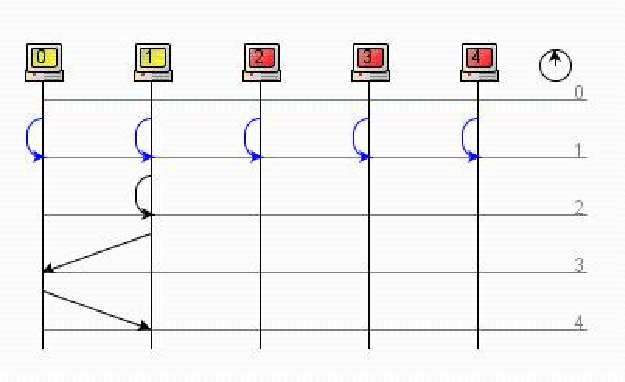
\includegraphics{images/p1ReadSeq.pdf}
	\caption{Bezeichnung der Abbildung}
	\label{a1}
\end{figure}

\begin{table} %[hbtp]
	\centering
		\begin{tabular}{l | l l l l}
		\textbf{Prozesse} & \textbf{Zeit} $\rightarrow$ \\
		\hline
			$P_{1}$ & $W(x)1$ \\
			$P_{2}$ & & $W(x)2$ \\
			$P_{3}$ & & $R(x)2$ & & $R(x)1$\\
			$P_{4}$ & & & $R(x)2$ & $R(x)1$\\
		\end{tabular}
	\caption{Bezeichnung der Tabelle}
	\label{t1}
\end{table}


\section{Mathematische Formel}\index{Formel}
Mathematische Formeln bzw. Formulierungen k�nnen sowohl im
laufenden Text (z.B. $y=x^2$) oder abgesetzt und zentriert im Text
erscheinen. Gleichungen sollten f�r Referenzierungen nummeriert
werden (siehe Formel \ref{gl-1}).
\begin{equation}
\label{gl-1}
e_{i}=\sum _{i=1}^{n}w_{i}x_{i}
\end{equation}

Entscheidungsformel:

\begin{equation}
\psi(t)=\left\{\begin{array}{ccc}
1 &  \qquad 0 <= t < \frac{1}{2} \\
-1 &  \qquad \frac{1}{2} <= t <1 \\
0 & \qquad sonst
\end{array} \right.
\end{equation}


Matrix:\index{Matrix}
\begin{equation}
A = \left(
\begin{array}{llll}
a_{11} & a_{12} & \ldots & a_{1n} \\
a_{21} & a_{22} & \ldots & a_{2n} \\
\vdots & \vdots & \ddots & \vdots \\
a_{n1} & a_{n2} & \ldots & a_{nn} \\
\end{array}
\right)
\end{equation}

Vektor:\index{Vektor} 

\begin{equation}
\overline{a} = \left(
\begin{array}{c}
a_{1}\\
a_{2}\\
\vdots\\
a_{n}\\
\end{array}
\right)
\end{equation}

\section{S�tze, Lemmas und Definitionen}\index{Satz}\index{Lemma}\index{Definition}

S�tze, Lemmas, Definitionen, Beweise,\index{Beweis} Beispiele\index{Beispiel} k�nnen in speziell daf�r vorgesehenen Umgebungen erstellt werden.

\begin{definition}(Optimierungsproblem)

Ein \emph{Optimierungsproblem} $\mathcal{P}$ ist festgelegt durch ein Tupel
$(I_\mathcal{P}, sol_\mathcal{P}, m_\mathcal{P}, goal)$ wobei gilt

\begin{enumerate}
\item $I_\mathcal{P}$ ist die Menge der Instanzen,
\item $sol_\mathcal{P} : I_\mathcal{P} \longmapsto \mathbb{P}(S_\mathcal{P})$ ist eine Funktion, die jeder Instanz $x \in I_\mathcal{P}$ eine Menge zul�ssiger L�sungen zuweist,
\item $m_\mathcal{P} : I_\mathcal{P} \times S_\mathcal{P} \longmapsto \mathbb{N}$ ist eine Funktion, die jedem Paar $(x,y(x))$ mit $x \in I_\mathcal{P}$ und $y(x) \in sol_\mathcal{P}(x)$ eine
Zahl $m_\mathcal{P}(x,y(x)) \in \mathbb{N}$ zuordnet (= Ma� f�r die L�sung $y(x)$ der Instanz $x$), und
\item $goal \in \{min,max\}$.
\end{enumerate}

\end{definition}

\begin{example} MINIMUM TRAVELING SALESMAN (MIN-TSP)
\begin{itemize}
\item $I_{MIN-TSP} =_{def}$ s.o., ebenso $S_{MIN-TSP}$
\item $sol_{MIN-TSP}(m,D) =_{def} S_{MIN-TSP} \cap \mathbb{N}^m$ 
\item $m_{MIN-TSP}((m,D),(c_1, \ldots , c_m)) =_{def} \sum_{i=1}^{m-1} D(c_i, c_{i+1}) + D(c_m,c_1)$ 
\item $goal_{MIN-TSP} =_{def} min$
\end{itemize}
\begin{flushright}
$\qed$
\end{flushright}
\end{example}

\begin{theorem} Sei $\mathcal{P}$ ein \textbf{NP}-hartes Optimierungsproblem.
Wenn $\mathcal{P} \in$ \textbf{PO}, dann ist \textbf{P} = \textbf{NP}.
\end{theorem}

\begin{proof} Um zu zeigen, dass \textbf{P} = \textbf{NP} gilt, gen�gt es
wegen Satz A.30 zu zeigen, dass ein einziges \textbf{NP}-vollst�ndiges
Problem in \textbf{P} liegt. Sei also $\mathcal{P}'$ ein beliebiges \textbf{NP}-vollst�ndiges Problem.

Weil $\mathcal{P}$ nach Voraussetzung \textbf{NP}-hart ist, gilt insbesondere
$\mathcal{P}' \leq_T \mathcal{P}_C$. Sei $R$ der zugeh�rige
Polynomialzeit-Algorithmus dieser Turing-Reduktion.
Weiter ist $\mathcal{P} \in$ \textbf{PO} vorausgesetzt, etwa verm�ge eines
Polynomialzeit-Algorithmus $A$. Aus den beiden
Polynomialzeit-Algorithmen $R$ und $A$ erh�lt man nun
leicht einen effizienten Algorithmus f�r $\mathcal{P}'$: Ersetzt man
in $R$ das Orakel durch $A$, ergibt dies insgesamt eine polynomielle
Laufzeit. 
%\begin{flushright}
$\qed$
% \end{flushright}
\end{proof}

\begin{lemma} Aus \textbf{PO} $=$ \textbf{NPO} folgt \textbf{P} $=$ \textbf{NP}.
\end{lemma}

\begin{proof} Es gen�gt zu zeigen, dass unter der angegeben
Voraussetzung KNAPSACK $\in$ \textbf{P} ist.

Nach Voraussetung ist MAXIMUM KNAPSACK $\in$ \textbf{PO},
d.h. die Berechnung von $m^*(x)$ f�r jede Instanz $x$ ist
in Polynomialzeit m�glich. Um KNAPSACK bei Eingabe
$(x,k)$ zu entscheiden, m�ssen wir nur noch $m^*(x) \geq k$
pr�fen. Ist das der Fall, geben wir $1$, sonst $0$ aus. Dies
bleibt insgesamt ein Polynomialzeit-Algorithmus. 
\begin{flushright}
$\qed$
\end{flushright}
\end{proof}

\section{Fu�noten}

In einer Fu�note k�nnen erg�nzende Informationen\footnote{Informationen die f�r die Arbeit zweitrangig sind, jedoch f�r den Leser interessant sein k�nnten.} angegeben werden. Au�erdem kann eine Fu�note auch Links enthalten. Wird in der Arbeit eine Software (zum Beispiel Java-API\footnote{\url{http://java.sun.com/}}) eingesetzt, so kann die Quelle, die diese Software zur Verf�gung stellt in der Fu�note angegeben werden.

\section{Literaturverweise}\index{Literatur}
Alle benutzte Literatur wird im Literaturverzeichnis angegeben\footnote{Dazu wird ein sogennanter bib-File, literatur.bib verwendet.}. Alle angegebene Literatur sollte mindestens einmal im Text referenziert werden\cite{Coulouris:02}.